\section{Машина Тьюринга. Вычисление словарных и числовых функций на машинах Тьюринга. Тезис Чёрча- Тьюринга.}
% ОБРАТИ ВНИМАНИЕ НА ТО, ЧТО В САМОМ НАЧАЛЕ ФАЙЛА ПОДКЛЮЧАЮСЯ + ТРОЕ (для
% графики); НИЧЕГО НЕ МЕНЯТЬ В ЭТОМ ГОВНОКОДЕ, рискуешь споткнуться о костыли,
% серьёзно,просто не трогай, я не знаю, как оно едет, но мне всё равно, уже 4
% утра.
\subsection*{Машина Тьюринга.}
\par Неформально опишем машину Тьюринга: пусть есть некоторое устройство, на
котором находится ''бесконечная'' лента, заполненная символами ''$\#$''
(пробелами) почти всюду.
На ленте в любой конечный момент времени записано конечное количество информации.

(тут должна быть таблица с лентой, но она уехала вниз)

\begin{wraptable}{r}{7cm}
	\begin{tabular}{ c|c|c|c|c|c|c|c|c } 
		\hline
		$\#$ & $\#$ & $S_{0}$ & $S_{1}$ & $S_{2}$ & ... & ... & $\#$ & $\#$ \\  \hline
	\end{tabular}
	\\
	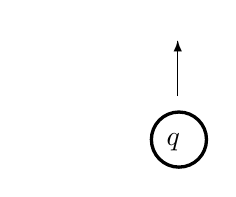
\begin{tikzpicture}
		\filldraw[color=white!100, fill=none, very thick](-5,-5) circle (0.4);
		\filldraw[color=black!100, fill=none, very thick](-3.5,-6) circle (0.35);
		\put(-100,-155){\vector(0,1){20}}
		\put(-104,-173){$q$}
	\end{tikzpicture}
\end{wraptable}

\par У устройства есть так называемая ''считывающая головка'',  находящаяся в одном из конечного множества
состояний $Q$ = \{ $q_{0}$, $q_{1}$, $q_{2}$, ...\}, где $q_{0}$ - конечное состояние, $q_{1}$ -- начальное
состояние. Можно понимать $Q$ как оперативную память. Головка считывает символы алфавита $\Sigma$ := \{$S_{0}$,
$S_{1}$,..., $S_{n}$\}, который называется ленточным алфавитом. 
\par Для машины есть ''инструкции'', которые говорят, что машине делать, когда ''она находится в состоянии $q_{i}$
и обозревает символ $S_{j}$''. Например, пусть $q_{i}S_{j} \to q_{i}S_{j}R$. Это значит, что наша машина,
находясь в состоянии $q_{i}S_{j}$, перейдёт в состояние $q_{i}S_{j}$ и считывающая головка сдвинется вправо (за это
отвечает $R$). Таким образом, любую команду мы можем записать пятёркой букв. 
\par Под программой $P$ будем подразумевать конечное множество команд такое, что для каждой пары $q_{i}S_{j}$ есть
ровно одна команда в P. Договариваются, что $q_{0}$ в команде писать необязательно: машина пришла в конечное
состояние и ей уже ничего не надо делать. Иногда считается, что если какая-то пара $q_{i}S_{j}$ не встречается в
инструкциях, то в этом случае машина останавливается. Существует  разновидность машин Тьюринга, в которых
нарушается однозначность соответствия пар состояния и команды. Они называются недетерминированными, но мы их в
курсе рассматривать не будем.
\par Под конфигурацией понимаем мгновенное описание того, что у нас происходит с машиной; будем записывать её как
тройку $XqY$, где $X, Y \subset \Sigma^*, q \in Q$. Головка машины смотрит на первый символ слева в слове $Y$.
\par Будем обозначать машину Тьюринга $M:=(Q, \Sigma, P, q_{0}, q_{1})$, где $Q$ -- конечное множество состояний,
$\Sigma$ -- ленточный алфавит, $P$ -- программа, $q_{0}$ -- конечное состояние, $q_{1}$ -- начальное состояние.
\begin{example}
	\par $\Sigma$ = \{\#, 0, 1 \}, $Q$ = \{$q_{0}$, $q_{1}$, $q_{2}$\}.  Программа:
	\par
	\begin{tabular}{ c c c} 
		$q_{1}\#$ & $\to\ $& $q_{1}\#R$ \\ $q_{1}0$ & $\to\ $& $q_{1}1R$ \\ $q_{1}1$ & $\to\ $& $q_{1}0R$ \\ $q_{2}\#$ & $\to\ $&
		$q_{0}\#L$ \\ $q_{2}0$ & $\to\ $& $q_{2}1R$ \\ $q_{2}1$ & $\to\ $& $q_{2}0R$ \\ 
	\end{tabular}
	\par
	\begin{wraptable}{r}{7cm}
		\begin{tabular}{ c|c|c|c|c|c|c|c|c } 
			\hline
			$\#$ & $\#$ & $0$  & $1$ & $0$ & $0$ & $0$ & $\#$ & $\#$ \\  \hline
		\end{tabular}
		\\
		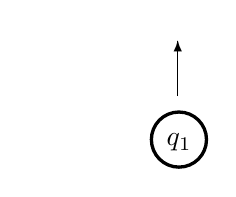
\begin{tikzpicture}
			\filldraw[color=white!100, fill=none, very thick](-5,-5) circle (0.4);
			\filldraw[color=black!100, fill=none, very thick](-3.5,-6) circle (0.35);
			\put(-100,-155){\vector(0,1){20}}
			\put(-104,-173){$q_{1}$}
		\end{tikzpicture}
	\end{wraptable}

	(а тут лента, которая еще ниже, а не эта)

	\par Что произойдёт при работе такой программы?  Из состояния $q_{1}$ машина перейдёт в состояние $q_{1}$, заменит
	первый символ слова, $0$, на $1$ и головка сдвинется вправо. Дальше из состояния $q_{1}$ машина перейдёт в
	состояние $q_{1}$, заменит второй символ слова, $1$, на $0$ и головка сдвинется вправо. Перейдёт ли машина
	когда-нибудь в состояние $q_{2}$? Нет. Она никогда не завершит работу (то есть не перейдёт в состояние
	$q_{0}$). Как же исправить программу, чтобы этого не происходило? 
	\par Давайте заменим $q_{1}0 \to\ q_{2}1R$, $q_{1}1 \to\ q_{2}0R$. Можно убедиться, что тогда программа будет
	работать, как мы и хотели: сначала получит слово 10111, затем завершит работу, встретив символ $\#$.
\end{example}
\subsection*{Вычисление словарных и числовых функций на машинах Тьюринга.}
\par Возникает естественный вопрос: а какие функции мы можем вычислять с помощью машин Тьюринга? Давайте
разбираться. Для начала, рассмотрим несколько примеров.
\par 
\begin{example}
	\par 1) Сложение можно реализовать, например, так: запишем числа $n-1$, $m-1$ черточками (число $n-1$ запишем $n$
	черточками, потому что мы хотим, чтобы 0 соответствовала одна черточка). Когда головка дойдёт до пробела,
	разделяющего эти числа, иначе говоря ''слова'' из чёрточек, она заменит его на черточку, а последнюю черточку
	из $m$ заменит на $\#$. Тогда количество черт не поменяется, однако же машина сможет прочитать сумму:
	\par $||...| \#|||...| \to ||...||||...|\#$
	\par $n, \#, m \to n,\ 1,\ m-1, \#$
	\par 2) Сравнивать два числа тоже очень просто: будем вычеркивать по одной четрочке из каждого числа. Как только
	одно из чисел будет состоять из одной черточки, то есть мы получили ноль, смотрим на другое: если к этому
	моменту в нём остались две или более чёрточки, то оно больше.
	\par 3) Умножить числа теперь не предствляется трудным: будем складывать столько раз, сколько потребуется. 
\end{example}
\par 
\begin{definition}
	Пусть $f\colon\Sigma^* \to\Sigma^*$ -- частичная функция. $f$ \textbf{вычислима машиной Тьюринга} $M=(Q,
	\Sigma_{M}, P, q_{0}, q_{1})$, если $\Sigma \subset\ \Sigma_{M}$ (то есть алфавит $\Sigma$ является
	подалфавитом $\Sigma_{M}$),\ $\# \notin \Sigma$ ("пробела"\ нет в алфавите $\Sigma$) и $M$ переводит
	конфигурацию $q_{1}X \mapsto q_{0}f(X)$, где $X, f(X) \in \Sigma^*$.
\end{definition}
\par Если $x \notin\dom(f)$, то $M$ на $q_{1}X$ не остановится.
\begin{definition} $f$ \textbf{вычислима}, если существует машина Тьюринга, которая её вычисляет.
\end{definition}

\begin{remark}
	\par С таким же успехом мы можем рассматривать $f: \mathbb{N} \times \mathbb{N} \to \mathbb{N}$. 
\end{remark}
\begin{remark}
	\par Композиция $f(g(x))$ вычислимых функций $f$, $g$ вычислима.
\end{remark}
\subsection*{Тезис Чёрча-Тьюринга}
\begin{theorem}[\textbf{Тезис Чёрча-Тьюринга}] Для любой алгоритмически вычислимой функции существует вычисляющая
	её значения машина Тьюринга.
\end{theorem}
Другими словами, любая интуитивно вычислимая функция является вычислимой по Тьюрингу.
